\documentclass[linenumbers,RNAAS,trackchanges]{aastex631}
\usepackage[utf8]{inputenc}
\usepackage{hyperref}           % hrefs
\usepackage{natbib}             % for bibliography
\usepackage{float}              % figure positioning
\usepackage{svg}                % used for SVG images
\usepackage{graphicx}           % used for non-SVG images
\usepackage{csvsimple}
% Search Query Metadata
\shorttitle{Golden Ratio Search Method on Action Potential Curve Fit Model}
\shortauthors{Ajaykumar, et al.}

% Hyperlink setup
\hypersetup{
colorlinks=true,
linkcolor=blue,
urlcolor=blue
}

\begin{document}
\title{Employing the Golden Ratio Search Method on an Action Potential Curve Fit Models of the Rat Sciatic Nerve}
% [] is for ORCiD
\correspondingauthor{}
\email{nikhitaajaykumar@utexas.edu, khernandez@utexas.edu, darryl.tran@utexas.edu}
\author{Nikhita Ajaykumar}

\author{Kayla Hernandez}

% or 
% \nocollaboration{0}

\author{Darryl Tran}
\affiliation{University of Texas at Austin\\
110 Inner Campus Drive\\
Austin, TX 78705}

% 250 word limit for abstract
\begin{abstract}
The minima and maxima of a function is referred to as the minimum or maximum point of a function. The points can be further classified as local, a minima/maxima within a specified range, or global, an absolute minima/maxima for the entire function. These are often used to optimize performance across various models or determine points of least/most activity. One such case is the analysis of neural activity. Neural activity is often measured and represented by electrical signals and transmission of neurochemical hormones released from neuron-neuron communication due to ease of measurement. Analysis of these signals and other derivatives can be used to identify areas of low activity in paralysis patients and can shed light on research to bring back normal function \cite{5333075}
. This paper reviews the technique of the golden ratio search method to optimally find the minima or maxima of a function. 
\end{abstract}

% Use astrothesaurus numbers in place of num
\keywords{Golden Ratio (1) --- Minima (2) --- Action Potential (3)}
\section{Introduction} \label{sec:intro}
The golden ratio is an incredibly important mathematical tool that was born in antiquity. Its properties have been studied in a variety of subjects. The golden ratio proportions have been applied in the construction and design of architecture and art to provide aesthetic harmony. It can be seen in naturally occurring objects, such as shell patterns. Additionally, the golden ratio can be applied in physics, math, and optimization problems.

The origin of the golden ratio began in Ancient Greece.\cite{stakhov_2014} It was first used in geometry to divide a line into its extreme and mean ratio\cite{stakhov_2014}. The golden ratio as a concept initially appeared in Euclid’s “Elements”, where Euclid provided various geometric proofs to define the ratio\cite{stakhov_2014}. However, Euclid likely gained the idea from previous mathematicians like Pythagoras and Hippasus who philosophized about harmonic proportions\cite{stakhov_2014}. Ideas from Euclid’s “Elements” persisted in the following centuries and were translated into many languages\cite{stakhov_2014}. German mathematician, Simon Jacobs, observed that Fibonacci’s sequence converges to the golden ratio in the 16th century\cite{stakhov_2014}. In the 18th century, a formula was developed that used the golden ratio to find the value of a Fibonacci number based on its placement in the sequence\cite{stakhov_2014}. Also in the 18th century, the term “golden section”, a synonym for the golden ratio, was coined by another German mathematician, Martin Ohm\cite{stakhov_2014}. 

The discoveries and applications of many great mathematicians and philosophers made way for the modern “harmonization of mathematics”, which led to the merger of mathematics with theoretical natural sciences, giving rise to great discoveries like the “quasi-crystal”\cite{stakhov_2014}. This harmonization also resulted in many applications of the golden ratio in “golden” theoretical physics and computer science. Examples in physics include optimization problems, like the application of an online golden section method-based loss minimization scheme for direct torque-controlled induction motor drive\cite{8709593}. In computer science, the golden ratio has been applied as an expansion of the Newton method and has been used in data mining and data analytics. The golden ratio search algorithm works to simply and effectively find local minima and maxima for nonlinear systems.

This paper will explore the golden ratio search algorithm in its application to finding the hyperpolarization point of an action potential model from a rat neuron\cite{5333075}. In the nervous system, the neuron is the fundamental unit of communication. Neurons can communicate through electrical impulses that occur from the spike of the action potential. The action potential occurs from a depolarization current that results in a more positive voltage within the neuron. Eventually, the neuron reaches a hyperpolarization stage which results in a more negative voltage than the neuron was previously at in the resting state. Eventually, the neuron returns back to its equilibrium potential or resting state voltage. The hyperpolarization stage is important so that impulse will not generate another action potential in the opposite direction. Determining the hyperpolarization point can give more insight into the stages of the action potential within a rat neuron and can possibly be used in the application of modeling long-term depression, where a neuron’s communication is inhibited by being in a constantly hyperpolarized state.
 
\
\section{Problem to be Solved} \label{sec:problem}
The development of a golden ratio search algorithm to find the hyperpolarization point (minima) on two models (see: Numerical Methods, equation 1 and equation 2) for the action potential of a neuron. 

\begin{figure}[H]
    \centering
    \includegraphics[scale=.75]{ModelR54.png}
    \caption{Graph of Model R-5/4  (Equation 1)}
    \label{fig:asa}
    \centering
    \includegraphics[scale=.75]{Model8P.png}
    \caption{Graph of Model 8-P  (Equation 2)}
    \label{fig:code}
\end{figure}

\section{Numerical Method} \label{sec:method}
Two equations were analyzed for the minimum: 
\\\begin{center}Equation 1 - R 5/4 Model:\end{center}
$$f(t) = \frac{a_1t^5 + a_2t^4 + a_3t^3 + a_4t^2 + a_5t + a_6}{t^4 + b_1t^3 + b_2t^2 + b_3t + b_4}$$ 
where $a_1 = -0.0345, a_2 = -0.021, a_3 = 0.025, a_4 = 0.023, a_5 = 0.002, a_6 = -0.0009, b_1 = 1.255, b_2 = 0.573, b_3 = 0.145,$ and $b_4 = 0.024, f(t)(t \in [-1.5,1])$ and
\\\begin{center}Equation 2 - 8-P Model:\end{center}
$$f(t) = -0.13t^8 + 0.13t^7 + 0.97t^6 - 0.77t^5 - 2.8t^4 + 1.7t^3 + 3.8t^2 - 1.9t - 1.2$$

The numerical method used to solve this problem is the golden ratio search for a minimum. The main idea is to start with an interval where the minimum occurs and make the interval smaller and smaller, thus narrowing in on the minimum until the interval is within a certain tolerance. 

Given a function and an interval, say $[x_1,x_4]$, where the minimum of the function occurs, two points are selected within the interval. We shall denote these $x_2$ and $x_3$. The first point, $x_2$, is selected by dividing the length of the interval by the golden ratio and subtracting that quotient from $x_4$. The second point, $x_3$, is selected by adding the same quotient, that is the interval length divided by the golden ratio, to $x_1$. Thus, point $x_3$ is $\displaystyle\frac{1}{\phi}$ of the way between the start of the interval and the end of the interval, and point $x_2$ is the reflection of $x_3$ across the midline of the interval. That is, points $x_2$ and $x_3$ share the same distance from the center of the interval, and they share the same distance from the endpoints of the interval. 

Next, the function is evaluated at points $x_1, x_2, x_3,$ and $x_4$. Because an interval where the minimum occurs was chosen, $f(x_2)$ or $f(x_3)$ is smaller than the function evaluated at the endpoints. 

If $f(x_2) < f(x_3)$, then the minimum is in the interval $[x_1, x_3]$. Should this be the case, $x_4$ is set to $x_3$ and $x_3$ is set to $x_2$. $x_2$ is then evaluated using the new interval $[x_1, x_3]$ and the method described above using the golden ratio. 

If it is not the case above, then the the minimum is in the interval $[x_2, x_4]$. So, $x_1$ is set to $x_2$ and $x_2$ is set to $x_3$. $x_3$ is then evaluated using the new interval $[x_2, x_4]$ and the method described above using the golden ratio. 

So long as $|x_1 - x_4|$ is greater than the tolerance, the process is repeated of of evaluating the function at the four points, determining where the minimum falls between, and reestablishing the four points.

Once $|x_1 - x_4|$ is less than or equal to the tolerance, the minimum is approximated as $0.5 * (x_2 + x_3)$.

The Python code for the implementation of this algorithm can be found in the appendix. 

\section{Data} \label{sec:data}
When applying the Golden Ratio Search method to both equations, the method closely approximated the minima within a 1.0 x ${10^6}$ tolerance at the tenth iteration, followed by a slight uptick before converging to the correct approximation. Figure 3 and 4. graphically shows the approximations against the iterations. 

\begin{figure}[H]
    \centering
    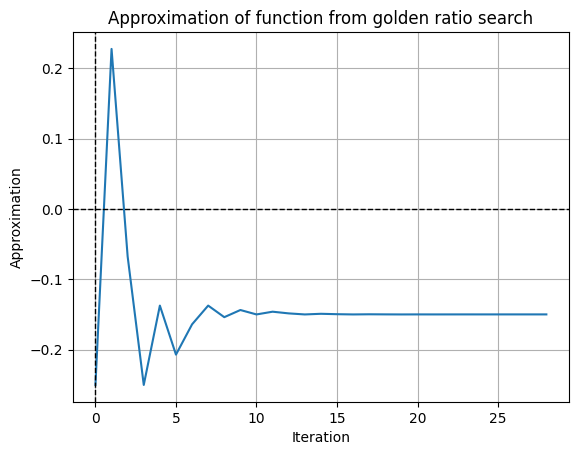
\includegraphics[scale=.75]{modelr54.png}
    \caption{Approximations given by Golden Ratio Search Method of Eq. 1}
    \label{fig:asa}
    \centering
    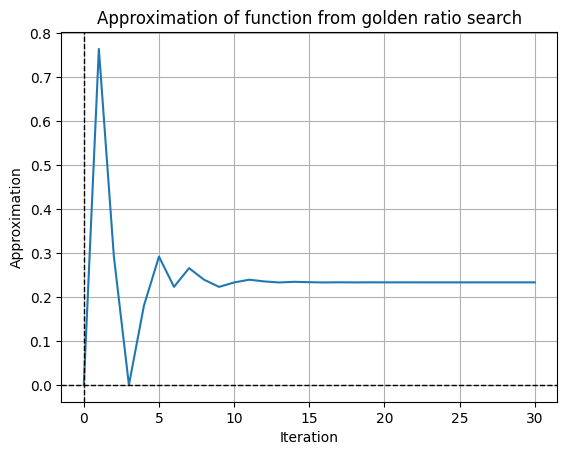
\includegraphics[scale=.75]{model8p.png}
    \caption{Approximations given by Golden Ratio Search Method of Eq. 2}
    \label{fig:code}
\end{figure}

The table below includes figures that more clearly reveal the approximations according to the Golden Ratio Search method. The first column is the number of iterations, the second column is the approximation given by the function, the third column is the error given by the approximation, and the fourth column is the slope between the current and previous approximation. The idea behind the fourth column is that as the approximation gets closer to the true minima, the slope should converge to a value of zero. The error was derived by taking the difference between the actual minima and the approximation. The first equation approximates the minima after 28 iterations and the second equation approximates the minima after 30 iterations. Table 1 corresponds to Figure 1 and Equation 1 while Table 2 corresponds to Figure 2 and Equation 2. 
\subsection{}
\begin{table}[]
\centering
\csvautotabular[respect all]{model-R54.csv}
\caption{Data representing the output per iteration for Equation 1 using the golden ratio search method}
\end{table}
\begin{table}
\centering
\csvautotabular[respect all]{model-R8P.csv}
\caption{Data representing the output per iteration for Equation 2 using the golden ratio search method}
\end{table}
\newpage


\section{Results} \label{sec:results}
The results illustrate that for Model 5/4 the hyperpolarization point is approximately 0.9999995849881831. For Model 8-P the hyperpolarization point is approximately 0.23315585755299917. 

After around 10 iterations for each model, the algorithm nearly converges to the correct approximation (see: Figure 5 and Figure 6). This demonstrates that there is no benefit as far as run-time goes for Model 8-P versus Model 5/4.  Model 5/4 was discovered to be the most accurate model for the action potential. The golden ratio search algorithm reveals that Model 5/4 is superior to Model 8-P in that the number of iterations is fewer. Model 5/4 produced 30 iterations, while Model 8-P produced 28 iteration (see: Table 1 and Table 2).


\begin{figure}[H]
    \centering
    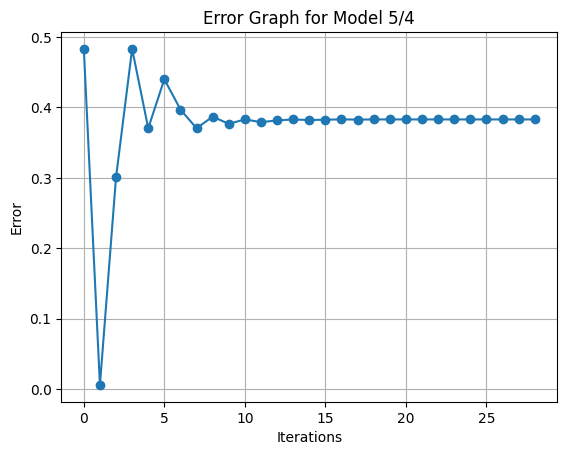
\includegraphics[scale=.75]{Error54.png}
    \caption{Error (final approximation - approximation at each iteration) vs Iteration graph for Model 5/4.}
    \label{fig:code}
    \centering
    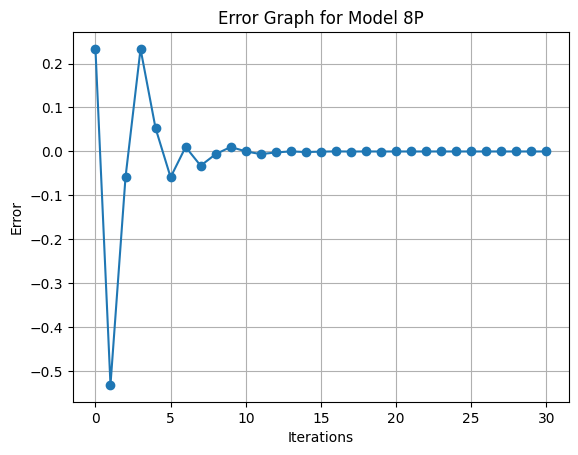
\includegraphics[scale=.75]{Error8P.png}
    \caption{Error (final approximation - approximation at each iteration) vs Iteration graph for Model 8-P.}
    \label{fig:code}
\end{figure}
\subsection{}
The figures above depict the slope of each approximation at each iteration. As expected, the slope eventually converges to 0 supporting the fact that the function correctly approximated the minima of each function after a certain amount of iterations. Figure 5 corresponds to Equation 1 and Figure 6 corresponds to Equation 2. 

\section{Conclusion} \label{sec:conclusion}
The results show that the golden ratio search works well in adequately predicting the local minima of nonlinear functions. The hyperpolarization points approximately match the graphical representation of each respective model (see: Figure 1 and Figure 2).

The method used does not indicate whether the minimum was global or local. In order to determine the type of minimum, the graph can be analyzed. By viewing the graph, it can be speculated where the interval with a local minimum versus a global minimum is contained. Furthermore, various intervals can be examined, and the minimum at each of these intervals can be gathered and then compared to find the minimum of the minimums, thus revealing a global minimum.

If a function has two variables, say $x$ and $y$, this method can be extended by considering the interval for $y$ in the same way done for $x$. The only difference would be checking a rectangular area to see where the minimum falls instead of an interval. Instead of having two cases where the minimum could be, four cases would have to be checked. Then when an area is reached that is within the tolerance, the position of the minimum is estimated at $x = 0.5 * (x_2 + x_3), y = 0.5 * (y_2, y_3)$.

The process for a function with more variables would take on the same idea prescribed above for two variables. The more variables, the more intervals to consider. Since the only consideration for a variable $\alpha$ is whether $\alpha_2$ or $\alpha_3$ is smaller, the total cases for a function of $n$ variables will be $2^n$.

Future analysis can be ran using Model 5/4 to identify areas of low activity in paralysis patients and can shed light on research to bring back normal function [1]. 


\section{Appendix} \label{sec:appendix}
\begin{figure}[H]
    \centering
    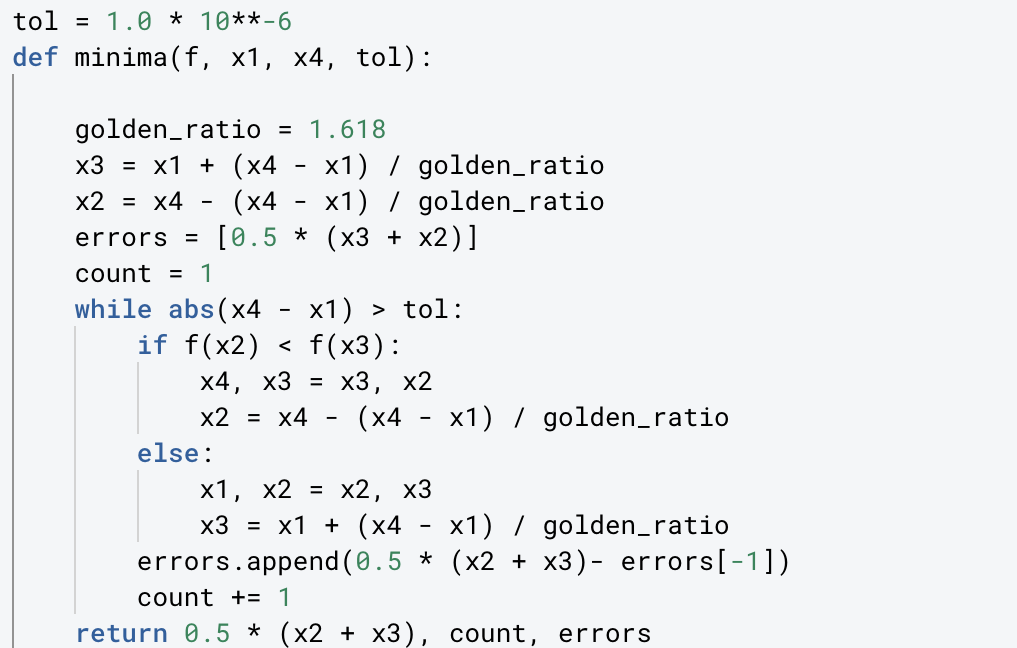
\includegraphics[scale=.75]{code.png}
    \caption{Python implementation of golden ratio search for minimum}
    \label{fig:code}
\end{figure}

\cite{5333075}
\cite{10.2307/2032161}
\cite{8709593}
\cite{stakhov_2014}

\newpage
\bibliographystyle{ieeetr}
\bibliography{citation.bib}

\section{Acknowledgements} \label{sec:acknowledgements}
We would like to express our gratitude to Brett Barkley and Dr. Shaymal Mitra for their guidance and lectures. 

We would also like to extend our gratitude to D. Chen, X. Lu, Z. Wang, and H. Pan for their contribution to the models used in this paper. 

\end{document}

